\documentclass{beamer}
\usetheme{CambridgeUS}
%\usecolortheme{dolphin} 
\usepackage[utf8]{inputenc}
\usepackage[spanish]{babel}
\usepackage{graphicx}

\title[Tecnologia]
{IPv6}
\subtitle{}
\author[Grupo 1] 
{Ignacio P\'erez Laborda\\B\'arbara Mart\'inez}
\institute[UB--FTI] 
{
  Facultad de Tecnolog\'ia Inform\'atica\\
  Universidad de Belgrano
}
\date[\today] 

\renewcommand{\thefootnote}{\roman{footnote}}

\begin{document}

%1
\begin{frame}


\includegraphics[height=0.2\textheight]{ub2.jpg} \hspace*{6cm}

\includegraphics[height=0.19\textheight]{FTI.jpg}  
\\[-0.1cm]
\titlepage


\end{frame}



%2
\begin{frame}
\frametitle{Que es IP? }
\framesubtitle{Introduccion}
\begin{enumerate}[$*$]
	\item En 1986 la National Science foundation  financió la construcción de una red para la conexión de sus computadoras. La NSF permitió a particulares conectarse a  dicha red.
	\item Estas redes existieron hasta 1993 cuando al año siguiente se puso un plan para reducir su influencia y aumentar la rentabilidad de los Internet Server Provider (ISP)
	\item El gobierno obligo a los ciudadanos a usar el modelo OSI pero aún así el modelo TCP/IP tuvo un gran crecimiento
		
\end{enumerate}
\end{frame}


%3




\begin{frame}
\frametitle{Que es IP? }
\framesubtitle{EL Protocolo IP}


	IP es un protocolo desarrollado por ARPANET para enrutar paquetes y comunicaciones de dispositivo a dispositivo de forma confiable. Vino de la mano de un paper presentado por Vinton Cerf y Robert Kahn.
\begin{enumerate}[$*$]

	\item IP se encarga de enrutar los paquetes y comunicaciones de dispositivo a dispositivo
	\item TCP garantiza confiabilidad en la comunicación de host a host
	\item Trabaja en capas pero esas mismas operan en conjunto. Esto se logra encapsulando los datos y formando un datagrama propio
	\item Promueve un servicio no orientado a la conexión no confiable y de mejor esfuerzo
	
\end{enumerate}
\end{frame}



\begin{frame}
\frametitle{El Estándar IPv4}
\framesubtitle{Aspectos Técnicos}


\begin{enumerate}[$*$]

	\item El estándar IPv4 utiliza un direccionamiento de 32 bits lo cual da una posibilidad de tan solo 
		4.294.967.296 posibles direcciones
	\item utiliza un sistema de 4 octetos expresados en decimal y separados por un punto. Identifican unívocamente equipo conectado a la red
	\item se han dividió las direcciones en clases
dando a una asignación llamada \textbf{direccionamiento con clases}
	
\end{enumerate}
\end{frame}

%
%\begin{frame}

%\frametitle{Que es IP? }
%\framesubtitle{El Protocolo IP}

%Estructura del datagrama
%\begin{enumerate}

	
	
%\item[Version] representa la version del estándar actualmente es cuatro en transición a 6.
%\item[Header Length] Tamaño del encabezado en múltiplos de 4 bytes.
%\item[DS/ECN] Usado para especificar el nivel del servicio, actualmente no se usa y solo esta
%presente para dar compatibilidad retroactiva.
%\item[Identification] Identificación única del datagrama de un host, se incremente con cada 
%datagrama.
%\item[Flags] El primero siempre queda en cero, los otros dos indican si se fragmenta o tiene varios
%fragmentos.
%\item[TTL] Especifica la cantidad de caminos que puede tomar un paquete hasta que se lo descarte, se
%utiliza para prevenir que el paquete quede para siempre dentro de un ciclo.
%\item[Protocol] Especifica el numero del protocolo superior.
%\item[Header Checksum] El checksum del header.
%\item[Options] Restricciones de seguridad, registro de ruta(se agrega la dirección del router por el 
%que pasa), marca de tiempo (por cada paso por router) y lista de rutas a pasar (por los únicos que 
%puede pasar o por los que debe pasar entre otros)
%\item[Padding] Se le agrega para asegurarse que tengo un tamaño de 4 bytes.		
%\end{enumerate}
%\end{frame}
%


\begin{frame}
\frametitle{Las falencias de IPv4}

\begin{enumerate}[$*$]

	\item Cupo limitado de direcciones asignables
	\item Falta de garant\'ias de seguridad, confiabilidad, movilidad y autenticidad
	\item Estos elementos podían incluirse mediante parches, pero a\'un as\'i no garantizaban el pleno desempeño de los mismos
	\item Si bien IPv4 posee un sistema de "servicios diferenciados"\footnote[1]{Diffserv: servicio que analiza varios flujos de datos en vez de conexiones únicas o reservas de recursos } no se garantizaba una calidad de servicio necesaria para cubrir la demanda actual en el mercado
\end{enumerate}



\end{frame}



%3
\begin{frame}
\frametitle{¿Qué es IPv6?}

Es la version 6 del protocolo de internet. La evolución del IPv4 y es un protocolo que soporta mas direcciones ($2^{128}$).\vspace{0.3cm}
\par Se solucionan problemas de direccionamiento y no son necesarias técnicas como el NAT\footnote{NAT (Network Address Translation - Traducción de Dirección de Red)}
% es un mecanismo utilizado por routers IP para intercambiar paquetes entre dos redes que se asignan mutuamente direcciones incompatibles} para proporcionar conectividad a todos los ordenadores/dispositivos de nuestra red.
\end{frame}

%4
\begin{frame}
\frametitle{Que propone IPV6}

\begin{enumerate}[$*$]
	
 	\item Direcciones Inagotables
	\item Simplificación de los encabezados:
	\item Seguridad
	\item Conexiones más eficaces
	\item Multicast
	\item Autoconfiguración
	\item Desaparición de los NAT
\end{enumerate}
\end{frame}
%5
\begin{frame}
\frametitle{Los Beneficios de IPv6}

\begin{enumerate}[$*$]
	
 \item Jerarquía de Direcciones
\item Direccionamiento mas sencillos
\item Autoconfiguración de Direcciones
\item Mejora en la Escalabilidad del Enrutamiento Multicast
\item La Nueva Cabecera del IPv6
\item Movilidad
\item Performance/Rendimiento



\end{enumerate}
Dado que este sistema mostró ciertas falencias para el rápido crecimiento de las conexiones y hosts
necesarios, se desarrollo las subredes y las mascaras de subred, pero aun así no es suficiente.

\end{frame}

%6
\begin{frame}
\frametitle{Los Beneficios de IPv6}
\framesubtitle{Jerarquía de Direcciones}


IPv6 divide las direcciones en distintos ámbitos definidos o limites en los cuales se delegan las 
direcciones.Cuenta con un agregado de un nivel superior TLA para la designación de un gran bloque de direcciones y la detección de la ruta de origen.\par Luego le sigue el NLA que rompe una porción del TDA  y se lo designa al SLA que se encarga de identificar subredes.

\end{frame}

%7
\begin{frame}
\frametitle{Los Beneficios de IPv6}
\framesubtitle{Direccionamiento mas sencillo}
El modelo IPv6 esta  caracterizado por tener una dirección de 128. Los primeros 64 bits están 
destinados a la numeración de red y los últimos 64 se utilizan para la numeración del host,
al tener 
128 bits es mucho mas variada la cantidad de direcciones que se pueden formar y también aumenta la 
seguridad de la red

\end{frame}

%8
\begin{frame}
\frametitle{Los Beneficios de IPv6}
\framesubtitle{Autoconfiguración de Direcciones}

\begin{enumerate}[$*$]
	
 \item Se puede decir que una red LAN es un grupo de 
maquinas y que cuando una nueva maquina ingresa a ese grupo, esta conectada y usan IPv6, se le 
enviara a esa maquina nueva un paquete de multidifusión, este paquete se destinara a la dirección 
de un ámbito local
\item Cuando el router ve que este paquete entra, este se puede responder con la 
dirección de red de la maquina nueva. La respuesta recibe el paquete y a su vez, lee el numero de 
red que el router tiene enviado. la maquina esta garantizada para tener la dirección única, 
porque el numero de red exclusivamente asignado por el numero de router de esa red.
\item Este mecanismo ahorra al usuario un montón de problemas tales como la configuración manual cuando el 
equipo se mueve de una red a otra, la realización de un seguimiento de las direcciones que se ha 
asignado y cuales están libres en un tiempo dado.


\end{enumerate}

\end{frame}



%9
\begin{frame}
\frametitle{Los Beneficios de IPv6}
\framesubtitle{Mejora en la Escalabilidad del Enrutamiento Multicast}
\begin{itemize}
\item Se copia  el archivo a enviar tantas 
veces como destinatarios existían y se los enviaba a cada uno.Esto resultaba inefectivo cuando se le mandaba el paquete a muchos usuarios en tiempo real.\par
\item Ipv6 implementará multidifusion, que es tomar  un conjunto de datos y enviarlo por una dirección de multidifusión
cuando se quiere enviar algo a multiples destinatarios, se asigna una dirección temporal de intervalo.\par
Esto ayuda a ahorrar ancho de banda y proporciona un envío eficaz.
\item  \textbf{Dirección anycast:} Es una dirección que envía paquetes en una relación uno a uno, decide a que equipo va a enrutar primero el paquete decidiendo cual es el equipo mas cercano.
 \end{itemize}
\end{frame}


%10
\begin{frame}
\frametitle{Los Beneficios de IPv6}
\framesubtitle{La Nueva Cabecera del IPv6}
La nueva cabecera que implementará el IPv6 solo tiene seis campos y dos direcciones.Las cualidades importantes que resaltan la sencillez de esta nueva cabecera son:
 \begin{enumerate}
\item \textbf{Formato Simplificado} Se simplifico la cantidad de campos de la cabecera,también se quito la 
variable de tamaño opcional.
\item \textbf{No hay checksum de la cabecera} fue eliminado el checksum de la cabecera
\item \textbf{Salteo de fragmentación del Procedure} En IPv6 solo el host puede fragmentar el paquete. Para ayudar al 
host, IPv6 incluye una función que encuentra la máxima unidad de transmisión(\textbf{MTU}) tamaño 
del origen hacia la transmisión.
\item \textbf{Cabeceras especiales} se agregaron las cabeceras de autenticación y la cabecera ESP

\end {enumerate}
\end{frame}

%11

\begin{frame}
\frametitle{Los Beneficios de IPv6}
\framesubtitle{Movilidad}
\begin{enumerate}
\item Las  IPv6 móviles son identificadas por una dirección hogareña.Cuando un host cambia de una subred a otra, se le asocia una dirección de atención.
\item El encuadernamiento es la asociación entre la dirección hogareña y la dirección de atención.
\item Cuando el dispositivo adquiere su dirección de atención , se le notifica al agente hogareño el cambio de estado con un msj de actualización de encuadernamiento
\item Se mantiene un mapeo entre ambas direcciones (cache de encuadernamiento)  
 \item Se enviara un mensaje 
de actualización al nodo de origen, se actualizará y enviará los paquetes subsiguientes directamente 
al nodo móvil a través de su atención  de la dirección.
\end{enumerate}
\end{frame}

%12
\begin{frame}
\frametitle{Los Beneficios de IPv6}
\framesubtitle{Performance/Rendimiento}

IPv6 incluye mejoras en el rendimiento y la escalabilidad.
\begin{enumerate}
\item Reducción de la traducción de direcciones En IPv6 la traducción de direcciones para superar 
las limitaciones de espacio no es necesaria
\item Reducción de gastos de enrutamiento  Reduce el enrutamiento exagerado
\item Ruta mas estable que  en IPv4 En IPv6, un solo proveedor puede agregar las rutas de muchas redes y permiten 
aislar la red del proveedor.
\item  Reducción de difusión IPv6  utiliza el descubrimiento de vecinos para realizar una función 
similar durante el proceso de configuración automática
 \item Multicast con ámbitos de enlace IPv6 contiene una dirección de multidifusión que contiene un 
campo de alcance que puede restringir los paquetes de multidifusión para el nodo, el enlace o la 
organización.
\item Cabecera Simplificada IPv6 Posee un encabezado aerodinámico de ocho campos de longitud 
fija. Estas cabeceras reducen la sobrecarga de la red. Además se elimina la existencia del checksum.

\end{enumerate}
\end{frame}


%13
\begin{frame}
\frametitle{Comparación IPv4 vs IPv6}
\framesubtitle{Estructura de dirección y Administración de direcciones}
IPv6 cuenta con una dirección de 128 bits de longitud y comprendido por un prefijo de subred y una 
interfaz de identificación, el identificador de interfaz deriva de la 
dirección MAC. Durante la configuración de la red IPv6 el nodo host remplaza su propia ID de 
interfaz por una ROM.
\par Para entender IPv6 hay que tener en claro la función de TLA ID Y NLA ID que apuntan a un direccionamiento jerárquico.
\par IPv4 en su lugar tiene unos bloques CIDR, cada uno compone de una o mas direcciones de clase C.El bloque CIDR no puede ser fácilmente agregado y se requiere una entrada en la tabla de enrutamiento , separada de un router.
\end{frame}


%14
\begin{frame}
\frametitle{Comparación IPv4 vs IPv6}
\framesubtitle{Comparación de cabeceras}
Sin embargo IPv6 cuenta con unos cabeceras adicionales que solo nombraremos, ya que los mas 
importantes fueron detallados en la sección anterior:
\begin{itemize}
\item Cabecera ``Salto a Salto" 
\item Cabecera de opción a destino
\item  Cabecera  de Ruteo
\item Cabecera de Fragmentación
\item Cabecera de Autenticación
\item  Cabecera ESP
\end{itemize}
Estas cabeceras tienen funciones especiales que mejoran el rendimiento de la dirección
\end{frame}

%15



\begin{frame}
\frametitle{Mecanismos de Transición}
\frametitle{Problemas en la Transición}
No se puede hacer un cambio abrupto entre un protocolo a otro porque : 
\begin{itemize}
\item La penetración en el mercado es muy baja 
\item Incompatibilidad de los protocolos
\item  No es factible apagar todos los servidores IPv4 porque tampoco es prudente dejar a la gente sin servicio

\end{itemize}
Se pensó en desplegar dos versiones del protocolo IPv4 en simultaneo para realizar paulatinamente la transición y a la vez  no quitarle la conexión a los usuarios.Esta solución se llama Dual stack.
Aun así no se cuenta con la cantidad suficiente de direcciones IP como para hacer eso.
\end{frame}

%16
\begin{frame}
\frametitle{Mecanismos de Transición}
\frametitle{Soluciones para la misma}
No se puede hacer un cambio abrupto entre un protocolo a otro porque: 
\begin{itemize}
\item Se pensó en desplegar dos versiones del protocolo IPv4 en simultaneo para realizar paulatinamente la transición y a la vez no quitarle la conexión a los usuarios.Esta solución se llama \textbf{Dual stack}.

\item \textbf{Tunneling}: utilización de túneles encapsulando IPV6 dentro de IPv4, permitiendo de esta forma atravesar redes que no manejan IPv6. Existen dos tipos de túneles, los manuales que  se configuran explícitamente y  los automáticos que se configuran automáticamente.
\item  \textbf{Traducción}: consiste en utilizar algún dispositivo en la red que convierta los paquetes de IPv4 a IPv6 y 
viceversa. Ese dispositivo tiene que ser capaz de realizar la traducción en los dos sentidos de 
forma de permitir la comunicación. 

\end{itemize}

\end{frame}

%18
\begin{frame}
\frametitle{ Anexo: Algunas empresas latinoamericanas que utilizan IPv6}
\centering
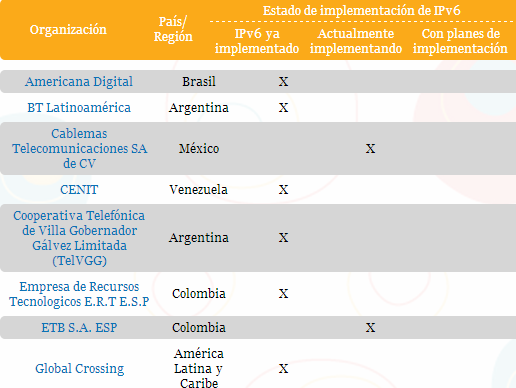
\includegraphics[height=.8\textheight]{empresas_ipv6_la.png}

\end{frame}

\end{document}
